\section{目的}
依據 \textit{AIC Lab.pdf} PDF 48--58 頁，涵蓋 Lab 5.A 未補償兩級運算放大器及 Lab 5.B Miller／RC 補償，並完成各項頻域、DC 與時域量測。使用由使用者另行提供的模型庫，供應電壓為 1.0 V。這是本次教學適配條件，並非模型額定電壓的認證；講義原製程的 3.3 V 圖表與數字不直接當作通過門檻。程式依講義拓樸重寫，原始程式僅作尺寸與缺漏的參考。

\section{Spec 對照}
S 為實際模擬，D 為推導／討論；PM<45 表示該原電容案例沒有達到講義建議的 45 度。
\small\begin{longtable}{p{.46\linewidth}p{.30\linewidth}p{.15\linewidth}}\toprule
要求與 PDF 頁碼 & 對應 deck／檢查 & 狀態 \\ \midrule\endhead
兩級開迴路增益與相位（48--50） & D01 & S+D \\
未補償 buffer 振盪與 PM 意義（50--51） & D01/C0,D05/C0 & S+D \\
Cc=2pF、串聯 Rc 的補償（52--54） & D01,D05/C1--2 & S+D; PM<45 \\
低頻增益、-3dB、unity、PM（54） & D01; 10pF adaptation & S+D \\
ICMR、反相十倍 output swing（54--55） & D03--04 & S+D \\
CMRR、PSRR+、PSRR-（56--57） & D02 & S+D \\
雙向 slew、settling（58） & D05 & S+D \\
\bottomrule\end{longtable}\normalsize


\section{電路與設計推導}
\[
 |A_0|\simeq\frac{g_{m2}}{g_{ds2}+g_{ds4}}\,
 \frac{g_{m7}}{g_{ds7}+g_{ds8}},\qquad
 \mathrm{PM}=180^\circ+\angle A(j2\pi f_u),\quad |A(j2\pi f_u)|=1.
 \]
 \[
 R_z\simeq1/g_{m7},\qquad
 |A(f_{3dB})|=|A(1\,\mathrm{Hz})|/\sqrt2,\qquad
 SR_{20-80}=\frac{0.6|\Delta V_o|}{t_{80}-t_{20}}.
 \]本次 $I_{ref}=10\,\mu$A，$L=0.3\,\mu$m；M1/M2、M3/M4、M5、M6、M7、M8 的 W 分別為 35、54、2.2、30、269、73 $\mu$m。$C_L=10$ pF 是主要條件，另列 1 pF 比較。開迴路以 DC 校準的小差動偏壓把輸出置於約 0.5 V，沒有利用外加伺服改變 AC 回路。第一級與第二級以實際操作點導數估得增益約 101.03、90.25，乘積約 9118，與實測 9088 相近；不是將每一元件視為理想平方律。

未補償以 $10^{-21}$ F 近似開路；C1 為 2 pF，C2 為 2 pF + 330 $\Omega$，C3 為另列的 10 pF + 330 $\Omega$ 適配，C4 為相同補償但 $C_L=1$ pF。實際 $1/g_{m7}\approx187.74\,\Omega$，所以 330 $\Omega$ 不是精確零點消除值。PDF 48 第一級增益的分母元件編號與圖不一致，本次使用第一級輸出節點上的 M2/M4。

\section{模擬設定}
使用 PrimeSim HSPICE S-2021.09 win64，基本溫度 27 $^\circ$C，\texttt{runlvl=5}、\texttt{accurate}，輸出 \texttt{.op/.print/.measure}。每個 \texttt{.alter} 先重設完整基準參數與溫度，防止前一案例殘留。實際工作已完成，未出現 error 或 failed 量測；模型仍有被抑制的警告訊息，因此不宣稱完全沒有 warning。公開 netlist 不含模型路徑，以下註解標示本機執行前必須設定的模型入口；模型檔與設定只保留本機：
\begin{verbatim}
* MODEL_SETUP_REQUIRED
\end{verbatim}
CSV 與數值摘要位於該 lab 的 \texttt{results/}；所有圖均由真實列印數據重繪，不是波形軟體畫面截圖。\texttt{manifest.json} 提供 spec 對照與案例定義。五份 deck 共 19 案例。AC 為 1 Hz--10 GHz、80 points/decade；相位先 unwrap，PM 取第一個向下 unity crossing。DC buffer 掃 0--1 V、1 mV 步距；反相級 $R_{in}=10$ k$\Omega$、$R_f=100$ k$\Omega$，$V_{ref}=0.65$ V，理想式 $V_o=7.15-10V_{in}$。輸入掃 0.55--0.75 V、0.2 mV 步距。有效追蹤定義為絕對誤差不超過 10 mV。脈衝為 0.60--0.75 V，1 ns 邊緣、1 $\mu$s 延遲，模擬 5 $\mu$s、最大 0.2 ns 步距。Settling 要求其餘觀察窗都在實測最終步階的 1\% 內。

\section{結果與規格檢查}
\begin{center}\small\begin{tabular}{lrrrr}\toprule
Case & $A_0$ (dB) & $f_{3dB}$ (kHz) & $f_u$ (MHz) & PM (deg) \\ \midrule
0 & 79.17 & 156.659 & 124.561 & -5.78 \\
1 & 79.17 & 10.718 & 63.272 & 25.10 \\
2 & 79.17 & 10.718 & 64.364 & 35.84 \\
3 & 79.17 & 2.269 & 20.295 & 80.59 \\
4 & 79.17 & 2.274 & 21.016 & 93.66 \\
\bottomrule\end{tabular}\end{center}

\begin{figure}[htbp]\centering
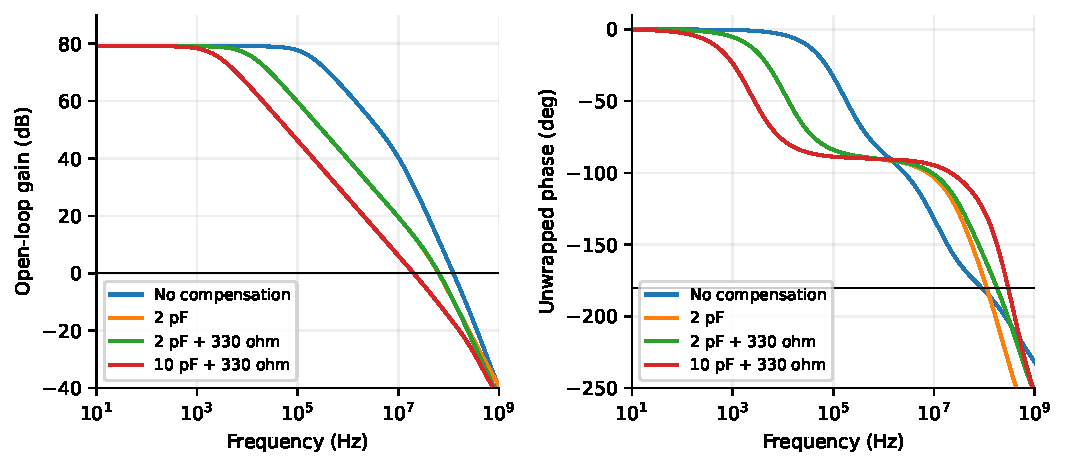
\includegraphics[width=\linewidth]{figures/compensation.pdf}
\caption{開迴路增益與展開相位。2 pF 與 2 pF + 330 歐姆在這些適配條件下均低於 45 度。}
\end{figure}
未補償低頻增益 79.17 dB、PM=-5.78 度；2 pF 為 25.10 度，加 330 $\Omega$ 為 35.84 度。加大到 10 pF 後為 80.59 度，unity 頻率降為 20.29 MHz。DC 靜態功耗約 479.85 $\mu$W。D02 在 1 Hz 的 CMRR、PSRR+、PSRR- 分別為 80.59、84.91、87.90 dB；均是名義匹配與指定輸入接地基準的結果。
\begin{center}\small\begin{tabular}{lrrrr}\toprule
Load & $V_{buf,min}$ & $V_{buf,max}$ & $V_{out,min}$ & $V_{out,max}$ \\ \midrule
Cap. only & 0.061 & 0.965 & 0.0117 & 0.9646 \\
100 k$\Omega$ & 0.061 & 0.964 & 0.0117 & 0.9643 \\
10 k$\Omega$ & 0.061 & 0.954 & 0.0116 & 0.9543 \\
\bottomrule\end{tabular}\end{center}
所有追蹤與輸出範圍單位為 V。Buffer 追蹤範圍同時受輸入共模與輸出擺幅限制，不能直接視為每顆 MOS 都飽和的獨立 ICMR。反相級的低頻增益幅值依負載為 9.9847、9.9827、9.9670，非精確 10。
\begin{center}\small\begin{tabular}{lrrrrrr}\toprule
Case & $SR_+$ & $SR_-$ & $t_{s,+}$ (ns) & $t_{s,-}$ (ns) & OS+ (\%) & OS- (\%) \\ \midrule
0 & 99.14 & -- & -- & -- & 91.56 & 67.42 \\
1 & 41.13 & 21.69 & 49.2 & 54.4 & 32.66 & 60.99 \\
2 & 41.02 & 21.48 & 31.2 & 37.8 & 21.16 & 49.48 \\
3 & 8.10 & 8.58 & 33.8 & 27.6 & 0.00 & 0.00 \\
\bottomrule\end{tabular}\end{center}

\begin{figure}[htbp]\centering
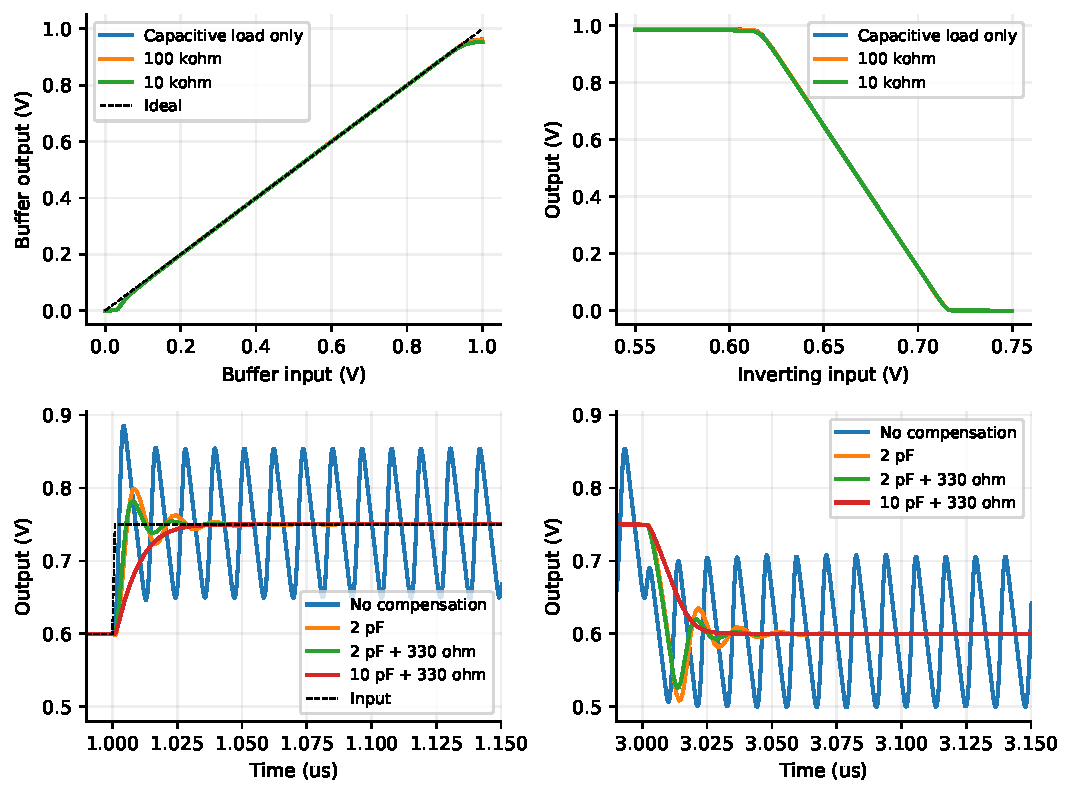
\includegraphics[width=\linewidth]{figures/closed_loop.pdf}
\caption{DC buffer／反相級轉移與上升、下降步階的局部放大。完整 5 微秒觀察窗保留在 CSV。}
\end{figure}
SR 單位為 V/$\mu$s，為指定步階的 20--80\% 平均斜率，不是所有幅度下的最大 slew-rate 保證。-- 表示觀察窗中未取得有效 crossing 或未穩定；未補償下降波形已有振盪，因此不能解讀為一個乾淨的單調下降 slew。10 pF + 330 $\Omega$ 的雙向 settling 分別為 33.8、27.6 ns，過衝均小於 0.001\%。

\section{討論}
共源第二級提供額外電壓增益，也帶來輸出極點與反相。改為 source follower 可降低輸出阻抗、提高驅動能力，但增益接近 1，總開迴路增益下降；cascode 可以增加增益，卻消耗擺幅與共模裕量。改拓樸時必須重建回授極性與完整 loop gain，不能沿用此 PM。

PM 表示 unity-loop-gain 處距離相位不穩定條件的餘量，並非任何負載與非線性狀態的穩定性保證。Miller 電容分裂極點、降低 dominant pole，通常降低 unity 頻率並改善 PM；串阻改變前饋零點。2 pF 沒有在此模型下重現講義的約 55 度，因此保留失敗結果並另列 10 pF 設計。PDF 54 將 -3 dB 說成半振幅；本報告以 $1/\sqrt2$ 幅值為定義，半幅其實約 -6.02 dB。多極點未補償電路的 $A_0f_{3dB}$ 約 1.42 GHz，與 124.56 MHz unity crossing 差很多，不能混稱同一 GBW。

\section{結論}
Lab 5.A/B 的電路與各量測皆完成。原 2 pF 補償未達 45 度；另列 10 pF + 330 歐姆在名義 10 pF 負載下達 80.59 度且兩方向可穩定。這不包含 corner、失配、佈局或矽晶驗證。

